\documentclass[a4paper,12pt]{article} 

%%% Работа с русским языком
\usepackage{cmap}                           % поиск в PDF
\usepackage{mathtext} 			 	       % русские буквы в формулах
\usepackage[T2A]{fontenc}               % кодировка
\usepackage[utf8]{inputenc}              % кодировка исходного текста
\usepackage[english,russian]{babel}  % локализация и переносы
\usepackage{wrapfig}

\usepackage{amsmath,amsfonts,amssymb,amsthm,mathtools} % AMS
\usepackage{euscript}	 % Шрифт Евклид
\usepackage{mathrsfs} % Красивый матшрифт
\usepackage{graphicx}%Вставка картинок правильная
\usepackage{float}%"Плавающие" картинки
\usepackage{wrapfig}%Обтекание фигур (таблиц, картинок и прочего)
\title{Лабораторная работа 2.3.1 

Получение и изучение вакуума}
\author{Кагарманов Радмир Б01-106}
\date{\today}

\begin{document}

\maketitle
\newpage

\paragraph{Цель работы:} 1) измерение объёмов форвакуумной и высоковакуумной частей установки; 2) определение скорости откачки системы в стационарном режиме, а также по ухудшению и по улучшению вакуума.
\paragraph{В работе используется:} вакуумная установка с манометрами: масляным, термопарным и ионизационным.

\paragraph{Экспериментальная установка}
Установка изготовлена из стекла и
состоит из форвакуумного баллона (ФБ), высоковакуумного диффузионного насоса (ВН), высоковакуумного баллона (ВБ), масляного (М) и
ионизационного (И) манометров, термопарных манометров ($\text{M}_1$ и $\text{M}_2$), форвакуумного насоса (ФН) и соединительных кранов $\text{K}_1, \text{K}_2, ..., \text{K}_6$.

\begin{figure}[h]
\centering
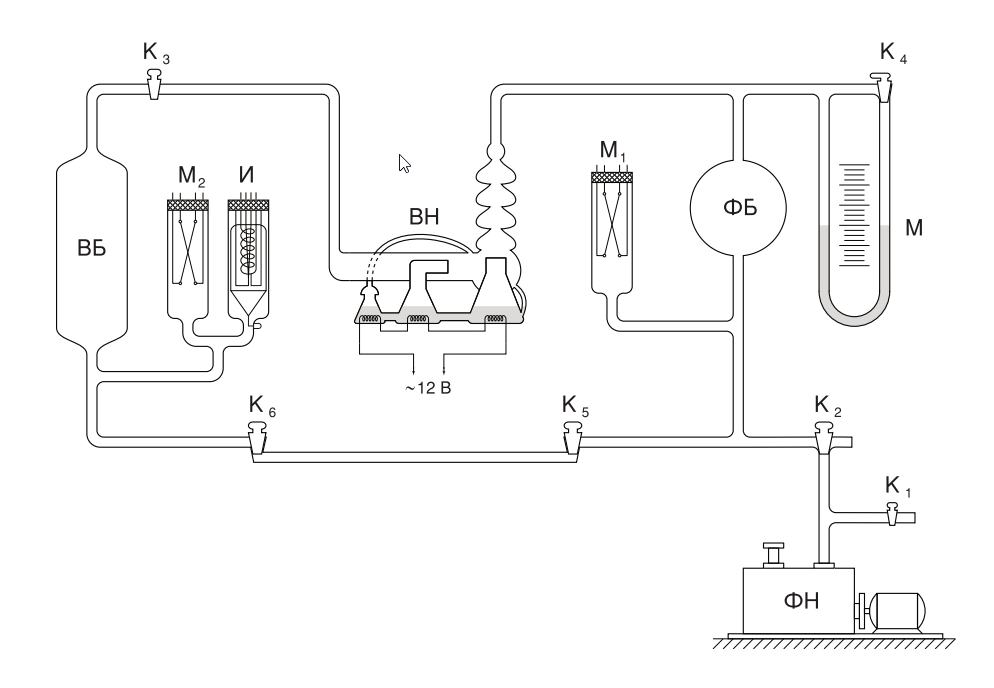
\includegraphics[width=0.8\linewidth]{1.png}
\caption{Экспериментальная установка}
\label{fig:mpr}
\end{figure}

Кран $\text{K}_1$ используется для заполнения форвакуумного насоса и вакуумной установки атмосферным воздухом. Во время работы установки он должен быть закрыт. Трёхходовой кран $\text{K}_2$ служит для соединения форвакуумного насоса с установкой или атмосферой. Кран $\text{K}_3$ отделяет
высоковакуумную часть установки от форвакуумной. Кран $\text{K}_4$ соединяет между собой колена масляного манометра. Он должен быть открыт во все время работы установки и закрывается лишь при измерении
давления в форвакуумной части. Краны $\text{K}_5$ и $\text{К}_6$ стоят по концам капилляра и соединяют его с форвакуумной и высоковакуумной частями
установки. 

\newpage

\begin{figure}[h]
\centering
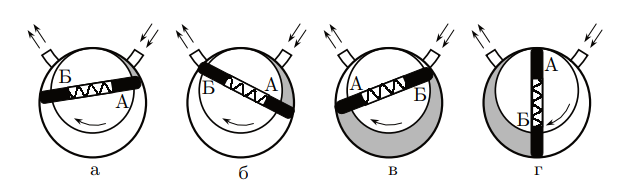
\includegraphics[width=0.8\linewidth]{2.png}
\caption{Схема действия ротационного двухпластинчатого форвакуумного насоса. В положениях «а» и «б» пластина «А» засасывает разреженный воздух
из откачиваемого объёма, а пластина «Б» вытесняет ранее захваченный воздух в атмосферу. В положениях «в» и «г» пластины поменялись ролями}
\label{fig:mpr}
\end{figure}

В цилиндрической полости массивного корпуса размещен эксцентрично ротор так, что он постоянно соприкасается своей верхней частью
с корпусом. В диаметральный разрез ротора вставлены две пластины,
раздвигаемые пружиной и плотно прижимаемые к поверхности полости.
Они разделяют объём между ротором и корпусом на две части.
Действие насоса ясно из изображённых на рис. 2 последовательных
положений пластин при вращении ротора по часовой стрелке. В положении «а» газ из откачиваемого объёма поступает в пространство между
пластиной «А» и линией соприкосновения корпуса и ротора. По мере
вращения это пространство увеличивается (рис. 2б), пока вход в него
не перекроет другая пластина «Б» (рис. 2в). После того как пластина
«А» пройдёт выходное отверстие и линию соприкосновения (рис. 2г),
лопасть «Б» будет сжимать следующую порцию газа и вытеснять его
через клапан в атмосферу.


\newpage


\begin{figure}[h]
\centering
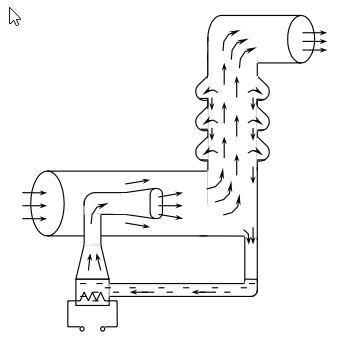
\includegraphics[width=0.8\linewidth]{3.png}
\caption{Экспериментальная установка}
\label{fig:mpr}
\end{figure}

Откачивающее действие диффузионного насоса основано на диффузии (внедрении) молекул разреженного воздуха
в струю паров масла. Попавшие в струю молекулы газа увлекаются ею
и уже не возвращаются назад. На прежнем их месте образуется пустота,
которая немедленно заполняется следующими порциями газа, увеличивая степень разрежения газа в окрестности струи и оказывая таким
образом сильное откачивающее воздействие на весь газ в откачиваемом
объёме. Скорость откачки диффузионных насосов в сотни и тысячи раз
превосходит скорость откачки форвакуумного насоса.
Устройство одной ступени масляного диффузионного насоса схематически показано на рис. 3 (в лабораторной установке используется
несколько откачивающих ступеней). Масло, налитое в сосуд А, подогревается электрической печкой. Пары масла поднимаются по трубе Б
и вырываются из сопла В. Струя паров увлекает молекулы газа, которые поступают из откачиваемого сосуда через трубку ВВ. Дальше смесь
попадает в вертикальную трубу Г. Здесь масло осаждается на стенках
трубы и маслосборников и стекает вниз, а оставшийся газ через трубу
ФВ откачивается форвакуумным насосом. Диффузионный насос работает наиболее эффективно при давлении, когда длина свободного пробега молекул воздуха примерно равна ширине кольцевого зазора между
соплом В и стенками трубы ВВ. В этом случае пары масла увлекают
молекулы воздуха из всего сечения зазора \\ 

\paragraph{Процесс откачки.} 

Производительность насоса определяется скоростью откачки $W$ (л/с): $W$ - это объём газа, удаляемого из сосуда при
данном давлении за единицу времени.
\begin{equation}
    VdP=(PW-\sum\limits_{i} Q_i)dt
\end{equation} 
$Q_i$ - это количество газа попадающего в систему в единицу времени через течи, насос и т.д. Левая часть этого уравнения равна убыли газа в откачиваемом объёме $V$, а правая определяет количество газа, уносимого насосом, и количество прибывающего вследствие перечисленных выше причин за время
$dt$. При достижении предельного вакуума (давление $P_\text{пр}$). Тогда $\frac{dP}{dt}=0$. Через уравнение (1) найдём скорость откачки:
\begin{equation}
    W=\frac{\sum\limits_{i}Q_i}{P_\text{пр}}
\end{equation}

Считая $Q_i$ и $W$ постоянными проинтегрируем уравнение (1):

\begin{equation}
    P-P_\text{пр}=(P_0-P_\text{пр})\text{exp}(-\frac{W}{V}t)
\end{equation}

Полная скорость откачки $W$, собственная скорость откачки насоса $W_{\text{н}}$ и проводимости элементов системы $C_1, C_2,...$ соотносятся согласно формуле (4):
\begin{equation}
    \frac{1}{W}=\frac{1}{W_\text{н}}+\frac{1}{C_1}+\frac{1}{C_2}+...
\end{equation}

\paragraph{Течение через трубу}
Характер течения газа существенно зависит от соотношения между размерами системы и длиной свободного
пробега молекул. При атмосферном давлении и даже при понижении
давления до форвакуумного длина свободного пробега меньше диаметра трубок и течение откачиваемого газа определяется его вязкостью,
т. е. взаимодействием его молекул. При переходе к высокому вакууму
картина меняется. Столкновения молекул между собой начинают играть меньшую роль, чем соударения со стенками.
Для количества газа, протекающего через трубу в условиях высокого вакуума, или, как говорят, в кнудсеновском режиме, справедлива формула:

\begin{equation}
    \frac{d(PV)}{dt}=\frac{4}{3}r^{3}\sqrt{\frac{2\pi RT}{\mu}}\frac{P_2-P_1}{L}
\end{equation}
Если труба соединяет насос и установку, то давлением $P_1$ у насоса можно пренебречь. Давление в сосуде $P = P_2$. Тогда имеем:
\begin{equation}
C_\text{тр} = \left(\frac{dV}{dt}\right)_\text{тр} = \frac{4r^3}{3l}\sqrt{\frac{2\pi RT}{\mu}}
\end{equation}
\newpage

\section*{Ход работы}

\paragraph{Определение объёмов форвакуумной и высоковакуумной частей установки}

\subparagraph{1.} Впустим в установку атмосферный воздух.
\subparagraph{2.}Запрём в капилляре $V_0=50$ $\text{см}^3$ воздуха при атмосферном давлении $P_\text{атм}=101000\pm 100$ Па
\subparagraph{3.}Подключим установку к форвакуумному насосу и откачаем установку до давления $10^{-2}$ торр
\subparagraph{4.}После открытия крана $\text{K}_5$ запертый воздух распространился по всей форвакуумной части. Измерим показания масляного манометра: \\
$h_1=34,4\pm 0,1$ см масл. ст, $h_2=9,0\pm 0,1$ см масл. ст. \\
$\sigma_{\Delta h_\text{фв}} = \sqrt{{\sigma_{ h_\text{1}}}^2 + {\sigma_{ h_\text{2}}}^2}\approx 1,1$\% \\
$\Delta h_{\text{фв}}= (25,4\pm 0,3)~ см~ масл. ~ст.$
\subparagraph{5.} Пользуясь законом Бойля-Мариотта, найдём объём форвакуумной части $V_\text{фв}$: \\
$V_\text{фв} = \frac{P_\text{атм}}{P_2}V_0$, где $P_2 = \rho_{масл}\Delta h_{\text{фв}}g$, $\rho_{масл}= 0,885\frac{\text{г}}{\text{см}^3}$ \\
$\sigma_{V_\text{фв}}=\sqrt{\sigma_{\Delta h_\text{фв}}^2 + \sigma_{P_\text{атм}}^2}\approx 1,1\%$ \\
$V_\text{фв} = (2,29\pm 0,03)~л$ 
\subparagraph{6.} Откроем кран $\text{K}_3$, чтобы газ заполнил высоковакуумную часть. Посчитаем её объём, как это сделали с фарвакуумной частью. \\
$h_1=30,1\pm 0,1$ см масл. ст, $h_2=13,9\pm 0,1$ см масл. ст. \\
$\sigma_{\Delta h_\text{вв}} = \sqrt{{\sigma_{ h_\text{1}}}^2 + {\sigma_{ h_\text{2}}}^2}\approx 0,8$\% \\
$\Delta h_{\text{вв}}= (16,2\pm 0,1)~ см~ масл. ~ст.$
\\
$V_\text{вв} = \frac{P_\text{атм}}{P_2}V_0$ \\
$\sigma_{V_\text{вв}}=\sqrt{\sigma_{\Delta h_\text{вв}}^2 + \sigma_{P_\text{атм}}^2}\approx 0,8\%$ \\
$V_\text{вв} = (1,30\pm 0,01)$ л

\section*{Получение высокого вакуума и измерение скорости откачки} 

\subparagraph{7.} После установки давления $10^{-2}$ мм рт. ст. в установке начинаем откачивать ВБ с помощью диффузионного насоса.
\subparagraph{8.} С помощью ионизационного манометра фиксируем предельное давление $P_\text{пр}=1,5 \cdot 10^{-4}$ мм рт. ст. 
\subparagraph{9.} Найдём скорость откачки по ухудшению и улучшению вакуума, для этого открывая и закрывая кран $К_3$ будем то подключать насос к объёму, то отключать его, при этом на видео зафиксируем показания манометра от времени и занесём полученные результаты в Таблицу 1 и построим графики необоходимых  зависимостей, для которых определим коэффициенты наклона прямых и их погрешности (с помощью МНК), полученные результаты также зафиксируем в Таблице 1. Так же запишем итоговое значение для коэффициента наклона прямых, которое является средним из двух полученных.


Сначала проведём вычисления для коэффициента $k$, полученного при улучшении вакуума (для этого мы строили графики зависимости $\ln ((P-P_0) / (P_0 - P_{пр}))$ от $t$). Поскольку $W = -kV_{вв}$, то $\varepsilon_W = \sqrt{\varepsilon_k^2 + \varepsilon_{V_{вв}}^2} \approx 1,4\%$, в результате имеем: $W = (7,92 \pm 0,11) ~ л /с.$
\subparagraph*{10.} Оценим величину потока газа  $Q_Н$. Для этого воспользуемся данными, полученными при ухудшении вакуума. А именно построим графики зависимости $P(t)$ и определим для них коэффициенты угла наклона прямой. Поскольку $V_{вв}dP = (Q_Д + Q_И) dt$ получим $)(Q_Д + Q_И) = kV_{вв} = (1.80 \pm 0.02)~ \cdot 10^{-5} ~торр \cdot л / c $ (Погрешность рассчитывается по формуле $\varepsilon =  \sqrt{\varepsilon_k^2 + \varepsilon_{V_{вв}}^2} \approx 0,8\%$). 
Используя формулу $Q_Н = P_{пр}W - (Q_Д + Q_И)$, а значит $\varepsilon_{Q_Н} =  \sqrt{\varepsilon_{P_{пр}W}^2 + \varepsilon^2} \approx 1,6\%$ получим, что: 
 
 $
 Q_Н = (9,29 \pm 0,15) \cdot 10^{-5} ~ торр \cdot л / с.
 $
 
 \section*{Вывод}
 В ходе данной лабораторной работы удалось проверить законы, в соответствии с которыми вакуум в установке ухудшается и улучшается, на графиках ухудшения хорошо видно, что зависимость линейная, но на графиках улучшения виден большой разброс. Также была изучена скорость откачки по ухудшению и улучшению вакуума. \\$W = (7,92 \pm 0,11) ~ л /с.$ \\
 $
 Q_Н = (9,29 \pm 0,15) \cdot 10^{-5} ~ торр \cdot л / с.
 $\\
 Были найдены объёмы форвакуумной и высоковакуумной частей установки: \\
 $V_\text{фв} = (2,29\pm 0,03)~л$ \\
$V_\text{вв} = (1,30\pm 0,01)$ л

\begin{table}[h!]
	\centering 
	\caption{Результаты измерений}
	\begin{tabular}{|l|l|l|l|l|l|l|l|} \hline 
		\multicolumn{4}{|c|}{Улучшение} & \multicolumn{4}{|c|}{Ухудшение} \\ \hline
		$P, \cdot 10^{-5}~ торр$ & $t, с$ &$P, \cdot 10^{-5}~ торр$ & $t, с$ &$P, \cdot 10^{-5}~ торр$ & $t, с$ &$P, \cdot 10^{-5}~ торр$ & $t, с$  \\ \hline
		75 & 0 & 76 & 0 & 15 & 0 & 15  & 0 \\ \hline 
		73 & 1 & 74 & 1 & 17 & 3 & 18 & 3 \\ \hline 
		67 & 2 & 70 & 2 & 21 & 6 & 23 & 6 \\ \hline 
		51 & 3 & 61 & 3 & 26 & 9 & 28 & 9 \\ \hline 
		39 & 4 & 49 & 4 & 31 & 12 & 33 & 12 \\ \hline 
		30 & 5 & 37 & 5 & 35 & 15 & 37 & 15 \\ \hline
		23 & 6 & 28 & 6 & 40 & 18 & 42 & 18\\ \hline 
		20 & 7 & 22 & 7 & 44 & 21 & 46 & 21 \\ \hline
		18 & 8 & 19 & 8 & 48 & 24 & 50 & 24 \\ \hline 
		17 & 9 & 17 & 9 & 53 & 27 & 54 & 27 \\ \hline
		15 & 10 & 16 & 10 & 56 & 30 & 58 & 30 \\ \hline 
		14 & 11 & 15 & 11 & 60 & 33 & 61 & 33 \\ \hline
		 &  & 14 & 12 & 64 & 36 & 65 &  36   \\ \hline
		 &  &  &  & 68 & 39 & 68 &  39     \\ \hline 
		 &  &  &  & 75 & 45 & 76  &  45     \\ \hline 
		\multicolumn{4}{|l|}{$k_1 = -6.196 ~  с^{-1}$} & \multicolumn{4}{|l|}{$k_1 = 1.387 ~ \cdot 10^{-5} ~торр \cdot с^{-1}$} \\ 
		
		\multicolumn{4}{|l|}{$k_2 = -5.989 ~ с^{-1}$}
		&\multicolumn{4}{|l|}{$k_2 = 1.376 ~ \cdot 10^{-5} ~торр \cdot с^{-1}$} \\ 
		
		
		\multicolumn{4}{|l|}{$k_{ср} = -(6.093 \pm 0.073) ~ с^{-1}$}
		&\multicolumn{4}{|l|}{$k_{ср} = (1.382\pm 0,006) ~ \cdot 10^{-5} ~ торр \cdot с^{-1}$} \\ 
		\hline
\end{tabular}
\end{table}
 
 \begin{figure} [h!]
	\caption{Ухудшение  вакуума 1}
	\centering 
	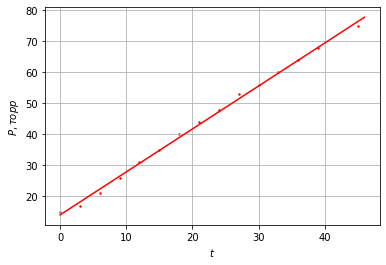
\includegraphics[scale=0.6]{Ухудшение1.png} 
\end{figure}

\begin{figure} [h!]
	\caption{Ухудшение  вакуума 2}
	\centering 
	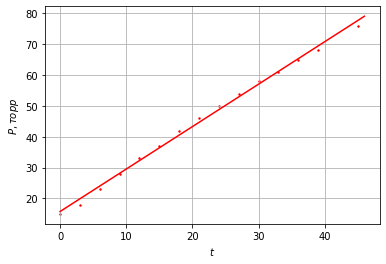
\includegraphics[scale=0.6]{Ухудшение2.png} 
\end{figure}

 \begin{figure} [h!]
	\caption{Улучшение вакуума 1}
	\centering 
	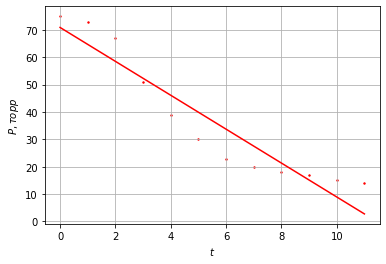
\includegraphics[scale=0.6]{Улучшение1.png} 
\end{figure}

\begin{figure} [h!]
	\caption{Улучшение  вакуума 2}
	\centering 
	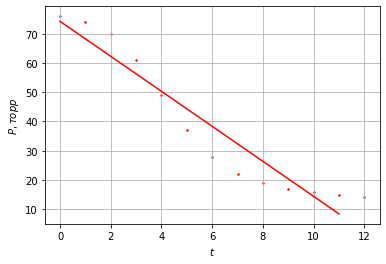
\includegraphics[scale=0.6]{Улучшение2.png} 
\end{figure}

\end{document}

